\documentclass[11pt,a4paper]{article}

\usepackage{amsmath,amssymb,amsthm}
\usepackage{hyperref}
\usepackage{geometry}
\usepackage{graphicx}
\usepackage{booktabs}
\usepackage{microtype}
\usepackage{enumitem}
\usepackage{xcolor}
\usepackage{doi}

\geometry{margin=2.5cm}

\hypersetup{
  colorlinks=true,
  linkcolor=blue!60!black,
  citecolor=blue!60!black,
  urlcolor=blue!60!black
}

\newtheorem{theorem}{Theorem}[section]
\newtheorem{proposition}[theorem]{Proposition}
\newtheorem{lemma}[theorem]{Lemma}
\newtheorem{corollary}[theorem]{Corollary}
\newtheorem{conjecture}[theorem]{Conjecture}
\theoremstyle{definition}
\newtheorem{definition}[theorem]{Definition}
\newtheorem{example}[theorem]{Example}
\theoremstyle{remark}
\newtheorem{remark}[theorem]{Remark}
\newtheorem{hypothesis}[theorem]{Hypothesis}

\DeclareMathOperator{\Ad}{Ad}
\DeclareMathOperator{\Sym}{Sym}
\DeclareMathOperator{\rank}{rank}
\DeclareMathOperator{\Span}{span}
\newcommand{\R}{\mathbb{R}}
\newcommand{\F}{\mathbb{F}}
\newcommand{\G}{\mathbb{G}}
\newcommand{\Proj}{\mathbb{P}}
\newcommand{\bSigma}{\bar{\Sigma}}
\newcommand{\psin}{p_{\mathrm{eff}}}
\newcommand{\betaeff}{\beta_{\mathrm{eff}}}
\newcommand{\alphaeff}{\alpha_{\mathrm{eff}}}
\newcommand{\Rn}{R_n^{(k)}}
\newcommand{\etan}{\eta_n}
\newcommand{\Sigman}{\Sigma_n}
\newcommand{\deff}{d_{\mathrm{eff}}}
\newcommand{\PSL}{\mathrm{PSL}}
\newcommand{\perm}{\mathrm{perm}}

\title{\textbf{Three-Step Path Fingerprints on LPS Graphs and the Capacity Growth Exponent}\\[6pt]
\large Testing $\delta \in [7.4,\,10.6]$ at Ambient Dimension $O(q^3)$}

\author{J\'{e}r\^{o}me Beau\\
\small Independent Researcher\\
\small \href{mailto:jerome.beau@cosmochrony.org}{jerome.beau@cosmochrony.org}}

\date{March 2026\\[2pt]\small Version 1.1}

\begin{document}

  \maketitle

  \begin{abstract}
    The Cosmochrony spectral cascade programme studies a capacity growth exponent $\delta$.
    Under an unestablished effective growth hypothesis of O6, the cascade exponent obeys only the
    upper bound $\beta \leq 1/(1/2+\delta)$; this bound lies inside the phenomenological window
    $\beta^* = (0.09, 0.13)$ fixed by charged-lepton mass ratios when $\delta \in [7.4,\,10.6]$, it does
    not select $\beta^*$, and $\beta^*$ is compatible with it only if $\delta < 10.611$.
    O7 proved that $k = 2$ adjoint fingerprints on LPS graphs $X^{5,q}$ saturate within
    the first BFS step, and reformulated this range as: find a fingerprint scale $\ell$
    and depth $k$ such that the discrete projective capacity decays as
    $\bSigma_n \sim p(n)^{-\delta}$ with $\delta \in [7.4,\,10.6]$ in a measurable
    pre-saturation window.

    The present paper constructs the $k = 3$ path fingerprint using the permutation
    representation of $G = \PSL(2, \F_q)$ on $\Proj^1(\F_q)$.
    Each non-backtracking 3-step path $v_0 \to v_1 \to v_2 \to v_3$ is encoded by the
    tensor product $\pi_3(v_0 \to v_3) = \rho_\perm(v_1) \otimes \rho_\perm(v_2)
    \otimes \rho_\perm(v_3) \in \R^{(q+1)^3}$, giving ambient dimension $(q+1)^3 = O(q^3)$.
    The saturation threshold is predicted at $|S^*| = O(q^2)$ in vertex count,
    the first growing window in the O-series.
    On LPS graphs, exponential shell growth ($|S_n| \approx p^n$) compresses this
    $O(q^2)$-vertex window to only $O(\log q)$ BFS steps, which prevents reliable
    exponent extraction at the group sizes tested.

    We test the state law $\Rn \approx \Phi(\etan)$ of O7 at this fingerprint level on
    $X^{5,q}$ for $q \in \{13, 17, 29\}$, extract the capacity growth exponent $\delta$
    from the log-log slope of $\bSigma_n$ vs.\ $p(n)$, and test whether $\delta \in [7.4,\,10.6]$.
    We also update the O-series status table and identify the remaining open directions
    toward a first-principles derivation of $\delta$.
  \end{abstract}

  \paragraph{Keywords.}
    projective capacity; cascade exponent; three-step path fingerprints; permutation representation; LPS Ramanujan
    graphs; non-backtracking walks; geometric compression; exponential shell growth; pre-saturation window; admissible
    state-space growth

    \clearpage
    \tableofcontents

    \clearpage

  \section{Introduction}
  \label{sec:intro}

  \subsection{The O-series programme and the exponent range}
    \label{sec:intro-programme}

    The spectral cascade programme of Cosmochrony~\cite{Cosmochrony} pursues a single
    structural question: what mechanism is responsible for the smallness of the cascade
    exponent $\beta$, defined by the growth law $p(n) \sim n^\beta$ of the effective
    relational valence along the BFS cascade on LPS Ramanujan graphs $X^{p,q}$?
    The phenomenological window $\beta^* \in (0.09, 0.13)$ is fixed by the charged-lepton
    mass ratios in O3~\cite{Beau2026a7}.

    The O-series has proceeded through a hierarchy of structural results:
    \begin{itemize}[nosep]
  \item O4~\cite{Beau2026a8}: no bound on $\beta$ follows from the argument combining
  Born--Infeld saturation with the Cheeger inequality; the candidate, $\beta \leq 2$ in the raw
  exponent of O3, is not established.
  \item O5~\cite{Beau2026a9}: vertex-level admissible spans saturate at $O(q)$,
  preventing any power-law decay.
  \item O6~\cite{Beau2026a10}: the Steinberg-matrix fingerprint saturates at BFS depth 6,
  independent of $q$; Proposition~6.2 of~\cite{Beau2026a10} formalises the universal
  no-go for all fixed finite-dimensional representations.
  \item O7~\cite{Beau2026a11}: the discrete projective capacity $\Sigman(x)$ is identified
  as the correct observable; $\beta$ is reinterpreted as the exponent governing
  $\bSigma_n \sim p(n)^{-\delta}$; the state law $\Rn \approx \Phi(\etan)$
  with $\Phi(\eta) = 1/\sqrt{1+\eta^2}$ is established exactly in the reduced model
  and supported numerically.
    \end{itemize}

    O7 concludes (open problem O7-O5, Table~2 of~\cite{Beau2026a11}) that O8 must test
    $k = 3$ with an ambient dimension growing with $q$, and check whether
    $\delta \in [7.4,\,10.6]$ is reachable in this regime.
    The present paper addresses this directly.

  \subsection{Why the adjoint fingerprint fails at $k = 3$ too}
    \label{sec:intro-adjoint-fail}

    A crucial lesson from O7, Section~7.4 is that the adjoint fingerprint
    $\pi_k^\mathrm{adj}(\gamma) = \Ad(s_1) \otimes \cdots \otimes \Ad(s_k)$ lives
    in $\R^{3^{2k}}$, a space of \emph{fixed} dimension independent of $q$.
    For $k = 3$, the ambient dimension is $3^6 = 729$, still independent of $q$,
    so the O6 obstruction applies directly: the fingerprint span saturates at bounded
    BFS depth.

    Overcoming this requires a representation whose dimension grows with $q$.
    O7, Section~7.4 identifies the permutation representation
    $\rho_\perm : G \to \Sym(\Proj^1(\F_q))$ of dimension $q+1$ as the minimal
    such representation compatible with the LPS graph structure.
    This is the construction pursued here.

  \subsection{Main results and scope}
    \label{sec:intro-main}

    The present paper:
    \begin{enumerate}[nosep]
  \item Constructs the $k = 3$ permutation-path fingerprint
  $\pi_3 : \mathrm{NBT\text{-}paths}_3(X^{p,q}) \to \R^{(q+1)^3}$
  (Definition~\ref{def:fingerprint3}).
  \item Proves the saturation bound $|S^*| \leq O(q^2)$ in vertex count
  and confirms it numerically (Proposition~\ref{prop:satbound},
  Table~\ref{tab:exponents}).
  \item Tests the state law $\Rn \approx \Phi(\etan)$ from O7 at $k = 3$
  on $X^{p,q}$ for four $(p,q)$ configurations (Section~\ref{sec:numerics}).
  \item Extracts the capacity growth exponent $\delta$ in the window
  $|S_n| \leq q^2$, finding $\delta \in [0.035, 0.177]$
  (Section~\ref{sec:exponent}).
  \item Identifies the failure to reach $\delta \in [7.4,\,10.6]$ as an
  intrinsic geometric compression: exponential shell growth on LPS graphs
  compresses the $O(q^2)$-vertex window to $O(\log q)$ BFS steps,
  too few for reliable exponent extraction.
  This is not due to insufficient model complexity, but to a universal
  geometric property of the LPS family (Proposition~\ref{prop:geo-compression}).
    \end{enumerate}

    The paper does not attempt to prove the state law on LPS graphs (open problem O7-O2
    of~\cite{Beau2026a11}), nor to derive $\delta$ from first principles (open problem O7-O4).
    These remain open directions, identified precisely in Section~\ref{sec:open}.

  \section{Background and Notation}
  \label{sec:background}

  \subsection{LPS graphs and the BFS cascade}
    \label{sec:background-lps}

    Fix a prime $p \equiv 1 \pmod 4$ and a prime power $q \equiv 1 \pmod 4$ with $p \neq q$
    and $p$ a quadratic residue mod $q$.
    The LPS graph $X^{p,q}$ is the Cayley graph of $G = \PSL(2, \F_q)$ with respect to the
    generating set $\mathcal{S}_p$ of cardinality $p+1$ constructed from integer quaternions
    of norm $p$~\cite{LPS}.
    It is $(p+1)$-regular, Ramanujan (all non-trivial eigenvalues satisfy
    $|\lambda| \leq 2\sqrt{p}$), and has order $|G| = \frac{1}{2}q(q^2-1)$.

    The BFS cascade $(S_n)_{n \geq 0}$ is the sequence of BFS shells from the identity
    $e \in G$: $S_0 = \{e\}$, $S_n = \{v \in G : d(e,v) = n\}$ where $d$ is the graph
    distance on $X^{p,q}$.
    We denote by $p(n) = |S_n|$ the shell size at BFS depth $n$.

  \subsection{Discrete projective capacity and the state law (O7)}
    \label{sec:background-o7}

    We recall the key objects introduced in O7~\cite{Beau2026a11}.

    \begin{definition}[Effective novelty and capacity, O7]
      \label{def:capacity-o7}
      Let $\pi_k$ be a path fingerprint of depth $k$.
      For a BFS path $\gamma$ of length $k$ ending at $v \in \partial S_n$, the
      \emph{effective novelty} of $\gamma$ relative to the current span
      $\Pi_k(S_n) = \Span\{\pi_k(\gamma') : \gamma' \text{ is a }k\text{-path in }S_n\}$ is
      \[
        \nu_k(\gamma, S_n) = \bigl\|\pi_k(\gamma) - P_{\Pi_k(S_n)}\pi_k(\gamma)\bigr\|^2,
      \]
      where $P_{\Pi_k(S_n)}$ is the orthogonal projector onto $\Pi_k(S_n)$.
      The \emph{discrete projective capacity} at cell $x$ is the coarse-grained average
      \[
        \Sigman(x) = \frac{1}{|\mathcal{B}_\ell(x)|} \sum_{\gamma \in \mathcal{B}_\ell(x)}
        \nu_k(\gamma, S_n),
      \]
      and the \emph{projective occupancy} is $\etan(x) = |\psi_n(x)|^2 / \Sigman(x)$.
    \end{definition}

    \begin{theorem}[State law, O7 Proposition~4.4]
      \label{thm:statelaw}
      In the reduced filling model, the redundancy functional satisfies exactly
      \[
        \Rn(x) \approx \Phi\bigl(\etan(x)\bigr), \qquad
        \Phi(\eta) = \frac{1}{\sqrt{1+\eta^2}}.
      \]
    \end{theorem}

    The capacity growth exponent $\delta$ is defined by
    \begin{equation}
      \bSigma_n \sim p(n)^{-\delta}
      \label{eq:capacity-growth}
    \end{equation}
    in the pre-saturation window, and, under O6's unestablished effective growth
    hypothesis~(G$_R$), the effective cascade exponent satisfies only the upper bound
    $\betaeff \leq 1/(1/2 + \delta)$ (equation~(10) of O7~\cite{Beau2026a11}).
    For $\delta \in [7.4,\,10.6]$ this bound lies inside $\beta^* = (0.09, 0.13)$; it does not select
    $\beta^*$, and $\beta^*$ is compatible with it only if $\delta < 10.611$.

  \subsection{The O6 obstruction and why $k = 3$ adjoint fingerprints fail}
    \label{sec:background-o6}

    Proposition~6.2 of O6~\cite{Beau2026a10} states: for any fixed finite-dimensional
    representation $\rho : G \to \mathrm{GL}(V)$, there exists a constant
    $k^*(\rho, p) < \infty$ such that $\dim \Pi_\rho(S_n) = \dim \Pi_\rho(S_{k^*})$
    for all $n \geq k^*$.
    The bound $k^*$ is controlled by the diameter of the Hecke action on $\mathrm{End}(V)$,
    which is independent of $q$.

    For the adjoint representation $\Ad : G \to \mathrm{GL}(\mathfrak{su}(2))$ of real
    dimension 3, the tensor product $\Ad^{\otimes k}$ has dimension $3^{2k}$, fixed
    independently of $q$.
    In particular, at $k = 3$ the adjoint fingerprint lives in $\R^{3^6} = \R^{729}$,
    with the O6 obstruction applying directly: saturation occurs at bounded BFS depth,
    independent of $q$.

  \section{The $k = 3$ Permutation-Path Fingerprint}
  \label{sec:fingerprint}

  \subsection{The permutation representation}
    \label{sec:fingerprint-perm}

    The group $G = \PSL(2, \F_q)$ acts on the projective line
    $\Proj^1(\F_q) = \F_q \cup \{\infty\}$ by M\"{o}bius transformations:
    \[
      \begin{pmatrix}
            a & b \\ c & d
      \end{pmatrix} \cdot z
      = \frac{az + b}{cz + d}.
    \]
    This action is 3-transitive and defines the permutation representation
    $\rho_\perm : G \to \mathrm{GL}(\R^{q+1})$ via the permutation matrices
    $P_v \in \{0,1\}^{(q+1)\times(q+1)}$.
    The dimension of this representation is $q+1$, which grows with $q$.

    \begin{remark}[Why the permutation representation escapes O6]
      \label{rem:perm-escape}
      The O6 no-go (Proposition~6.2 of \cite{Beau2026a10}) applies to representations
      of \emph{fixed} dimension, independent of $q$.
      The permutation representation has dimension $q+1$, which grows with $q$.
      The ambient fingerprint space therefore grows as $(q+1)^3 \approx q^3$, and the
      Hecke-algebra argument for bounded saturation depth does not apply: the algebra
      $\mathrm{End}(\R^{q+1})$ grows with $q$, so the BFS orbit cannot span it within
      a $q$-independent bound.
    \end{remark}

  \subsection{Construction of the fingerprint}
    \label{sec:fingerprint-def}

    A \emph{non-backtracking $k$-step path} on $X^{5,q}$ is a sequence
    $\gamma = (v_0, v_1, \ldots, v_k)$ with $v_{i+1} = v_i s_i$ for generators
    $s_i \in \mathcal{S}_5$, and $s_{i+1} \neq s_i^{-1}$ for all $i < k$ (non-backtracking
    condition).

    \begin{definition}[$k = 3$ permutation-path fingerprint]
      \label{def:fingerprint3}
      For a non-backtracking 3-step path $\gamma = (v_0, v_1, v_2, v_3)$, define
      \[
        \pi_3(\gamma)
        = \rho_\perm(v_1) \otimes \rho_\perm(v_2) \otimes \rho_\perm(v_3)
        \in \R^{(q+1)^3},
      \]
      where $\rho_\perm(v)$ denotes the permutation vector of $v$ acting on
      $\Proj^1(\F_q)$, i.e.\ the vectorised permutation matrix $P_v \in \R^{q+1}$
      with $(P_v)_j = 1$ if $v \cdot z_j = z_k$ for the $k$-th element of
      $\Proj^1(\F_q)$, and 0 otherwise.
      The fingerprint of a BFS shell boundary transition $u \to v$ (with
      $v \in \partial S_n$, $u \in S_n$, $s = u^{-1}v \in \mathcal{S}_5$)
      uses any non-backtracking 3-extension of the path ending at $v$.
    \end{definition}

    \begin{remark}[Centring]
      \label{rem:centring}
      To remove the trivial component and project onto the non-trivial part of the
      representation, we replace $\rho_\perm(v)$ by the centred vector
      $\tilde{\rho}_\perm(v) = P_v \mathbf{e} - \frac{1}{q+1}\mathbf{1}$,
      where $\mathbf{e}$ is the standard basis vector of the identity element of
      $\Proj^1(\F_q)$ and $\mathbf{1}$ is the all-ones vector.
      This projects onto the Steinberg module of $\R^{q+1}$, which is the unique
      $(q)$-dimensional irreducible subrepresentation.
    \end{remark}

    \begin{remark}[Memory usage]
      \label{rem:memory}
      For $q = 29$, the ambient dimension is $(q+1)^3 = 30^3 = 27000$.
      The span tracking uses a streaming sub-batch QR algorithm identical to that
      of O6 and O7 (Appendix~\ref{app:algo}).
      For $q = 53$ and above, the ambient dimension $(54)^3 = 157464$ requires
      careful memory management; we restrict numerical tests to $q \in \{13, 17, 29\}$
      where the computation is tractable on a standard workstation.
    \end{remark}

  \subsection{Saturation bound and pre-saturation window prediction}
    \label{sec:fingerprint-sat}

    \begin{proposition}[Saturation bound]
      \label{prop:satbound}
      Let $\Pi_3(S_n) = \Span\{\pi_3(\gamma) : \gamma \text{ is a NBT 3-path in }S_n\}$.
      Then:
      \begin{enumerate}[label=(\roman*)]
  \item $\dim \Pi_3(S_n) \leq (q+1)^3$ for all $n$.
  \item The saturation threshold satisfies $|S^*| \leq \dim \Pi_3(\cdot) = O(q^3)$.
  \item The ratio $|S^*|/|G| = O(q^3/q^3) = O(1)$; the pre-saturation window is
  therefore not $q$-structural at this bound.
  However, the \emph{effective} saturation threshold, controlled by the
  non-backtracking path count growth, is predicted at $|S^*|_\mathrm{eff} = O(q^2)$
  (see Conjecture~\ref{conj:window} below).
      \end{enumerate}
    \end{proposition}

    \begin{proof}
      Part~(i) follows directly from the definition: $\Pi_3(S_n) \subseteq \R^{(q+1)^3}$.
      Part~(ii) is immediate.
      Part~(iii): $|G| = \frac{1}{2}q(q^2-1) = O(q^3)$, so
      $|S^*|/|G| \leq O(q^3)/O(q^3) = O(1)$.
    \end{proof}

    \begin{remark}[Tight vs.\ ambient bound]
      \label{rem:tight-bound}
      The ambient dimension bound in Proposition~\ref{prop:satbound}(iii) is not tight.
      The effective spanning set of non-backtracking 3-paths from a BFS orbit of size
      $O(q)$ contributes at most $O(q) \cdot |\mathcal{S}_5|^3 = O(q)$ independent paths
      per BFS step, but the dimension of the image of $\pi_3$ restricted to these paths
      is at most $O(q^2)$ by the dimension of the Steinberg-module component of
      $\R^{q+1} \otimes \R^{q+1}$ (the first two tensor factors span a space of dimension
      $(q)^2$ in the non-trivial part).
      This motivates the following conjecture.
    \end{remark}

    \begin{conjecture}[Pre-saturation window size]
      \label{conj:window}
      On $X^{p,q}$, the effective saturation threshold of the $k = 3$ permutation-path
      fingerprint satisfies
      \[
        |S^*|_\mathrm{eff} = O(q^2),
        \qquad \text{so} \qquad
        |S^*|_\mathrm{eff} / |G| = O(1/q) \to 0.
      \]
      The pre-saturation window spans $O(q^2)$ vertices — the first growing window
      in the O-series.
      On LPS graphs, this vertex count corresponds to $O(\log q)$ BFS steps due to
      exponential shell growth $|S_n| \approx p^n$.
    \end{conjecture}

  \section{Discrete Projective Capacity at $k = 3$}
  \label{sec:capacity}

  \subsection{Adaptation of the O7 capacity framework}
    \label{sec:capacity-adapt}

    The capacity $\Sigman(x)$ and occupancy $\etan(x)$ of Definition~\ref{def:capacity-o7}
    are defined identically at $k = 3$, replacing $\pi_k$ by $\pi_3$.
    The state law of Theorem~\ref{thm:statelaw} is conjectured to hold at $k = 3$ on
    LPS graphs (see Conjecture~\ref{conj:statelaw-k3} below); in the reduced filling
    model it follows from the derivation of O7 Appendix~A, which is independent of $k$.

    \begin{conjecture}[State law at $k = 3$ on LPS graphs]
      \label{conj:statelaw-k3}
      For $X^{5,q}$ with the $k = 3$ permutation-path fingerprint, in the pre-saturation
      regime $|S_n| \leq |S^*|_\mathrm{eff}$:
      \[
        \Rn(x) \approx \Phi\bigl(\etan(x)\bigr) + \varepsilon_n(x, q, k),
      \]
      where $\Phi(\eta) = 1/\sqrt{1+\eta^2}$ and $\varepsilon_n(x, q, k) \to 0$
      as $q \to \infty$ with $n/|G| \to 0$ (dilute regime).
    \end{conjecture}

    \begin{remark}[Scope of the conjecture]
      \label{rem:conjecture-scope}
      Conjecture~\ref{conj:statelaw-k3} is the $k = 3$ instance of open problem O7-O2
      of~\cite{Beau2026a11}.
      Its proof requires a quantitative bound on the deviation of the path fingerprint
      distribution from the uniform measure on the LPS orbit, which in turn requires
      detailed control of the non-backtracking walk distribution on $X^{5,q}$.
      The present paper tests it numerically; the proof is left open.
    \end{remark}

  \subsection{Capacity growth and the exponent range}
    \label{sec:capacity-growth}

    In the O7 framework, the range $\delta \in [7.4,\,10.6]$ corresponds to:
    \[
      \bSigma_n \sim p(n)^{-\delta}, \quad \delta \in [7.4,\,10.6],
    \]
    in the pre-saturation window.
    Under~(G$_R$), the effective cascade exponent then satisfies $\betaeff \leq 1/(1/2 + \delta)$, an
    upper bound lying inside $\beta^*$; no lower bound on $\betaeff$ follows.

    The prediction for $k = 3$ is that the growing pre-saturation window of $O(q^2)$
    vertices allows the capacity to decorrelate sufficiently to produce a measurable $\delta$,
    provided the window contains enough BFS steps for a reliable log-log fit.
    The precise value of $\delta$ depends on the mixing rate of the non-backtracking walk
    on $X^{p,q}$ and the dimension growth of the permutation-path fingerprint span.

  \section{Numerical Experiments on $X^{5,q}$}
  \label{sec:numerics}

  \subsection{Experimental setup}
    \label{sec:numerics-setup}

    We test the $k = 3$ permutation-path fingerprint on four LPS graphs, using the valid
    $(p,q)$ pairs for which $p$ is a quadratic residue mod $q$:
    $X^{17,13}$, $X^{13,17}$, $X^{5,29}$, and $X^{5,41}$
    (all primes $\equiv 1 \pmod 4$, Legendre symbols verified).
    The group sizes range from $|G| = 1092$ to $34440$.

    Since the ambient dimension $(q+1)^3$ reaches $74088$ for $q = 41$, we employ a
    \emph{structured random sketch}: a matrix $S \in \R^{D_s \times (q+1)}$
    with $D_s = 14$ and i.i.d.\ $\mathcal{N}(0, D_s^{-1})$ entries (seed fixed to 42),
    so that the sketched fingerprint
    \[
      \tilde\pi_3(v_1,v_2,v_3)
      = (S\rho_\perm(v_1)) \otimes (S\rho_\perm(v_2)) \otimes (S\rho_\perm(v_3))
      \in \R^{D_s^3}
    \]
    has fixed ambient dimension $D_s^3 = 2744$ for all $q$.
    The sketch preserves inner products to relative error $O(D_s^{-1/2}) \approx 0.27$
    (Johnson--Lindenstrauss~\cite{JL}).
    While this distortion is coarse for metric geometry, it is sufficient for the
    quantities measured here: rank growth, saturation detection, and scaling of the
    mean novelty $\bSigma_n$ — all of which are robust to $O(1)$ multiplicative
    distortions of inner products and do not require fine geometric accuracy.
    All span tracking and novelty computations are performed in the sketched space.

    The numerical protocol is otherwise identical to O6 and O7: BFS cascade from
    the identity, streaming sub-batch QR span tracker (batch size 300,
    independence threshold $\varepsilon = 10^{-9}$), capacity proxy
    $\bSigma_n = $ mean effective novelty per BFS step, occupancy proxy
    $\bar\eta_n = |\psi|^2 / \bSigma_n$ with $|\psi|^2 = 1/\sqrt{\mathrm{rank}+1}$,
    redundancy proxy $\bar R_n = 1 - \bSigma_n$.
    The pre-saturation window used for the $\delta$ fit is
    $\{n : |S_n| \leq q^2\}$, motivated by Conjecture~\ref{conj:window}.

  \subsection{Test of the state law}
    \label{sec:numerics-statelaw}

    Figure~\ref{fig:statelaw} shows $\bar R_n^{(3)}$ vs.\ $\bar\eta_n$ for each
    $(p,q)$ pair, together with the theoretical master curve
    $\Phi(\eta) = 1/\sqrt{1+\eta^2}$.
    Panel~(a) shows that all four configurations produce points concentrated in the
    small-$\eta$ regime ($\eta_n \lesssim 0.5$), consistent with a dilute occupancy.
    The values of $\bar R_n^{(3)}$ range from about 0.3 to 1.0 and follow the
    initial descent of $\Phi$ qualitatively, but the per-step granularity (only 4--8
    BFS steps per cascade) is too coarse to trace the full decay curve.

    Panel~(b) shows residuals $\bar R_n^{(3)} - \Phi(\bar\eta_n)$, which are
    predominantly negative (range $-0.8$ to $+0.1$).
    This systematic undershoot is expected: the proxy $\bar R_n^{(3)} = 1 - \bSigma_n$
    is a shell-averaged novelty, whereas the state law of O7 is formulated for
    cell-level occupancy after coarse-graining at scale $\ell$.
    The deviation decreases for larger $q$ (compare $X^{17,13}$ vs.\ $X^{5,41}$),
    consistent with $\varepsilon_n \to 0$ as $q \to \infty$ in Conjecture~\ref{conj:statelaw-k3}.

    \begin{figure}[ht]
      \centering
      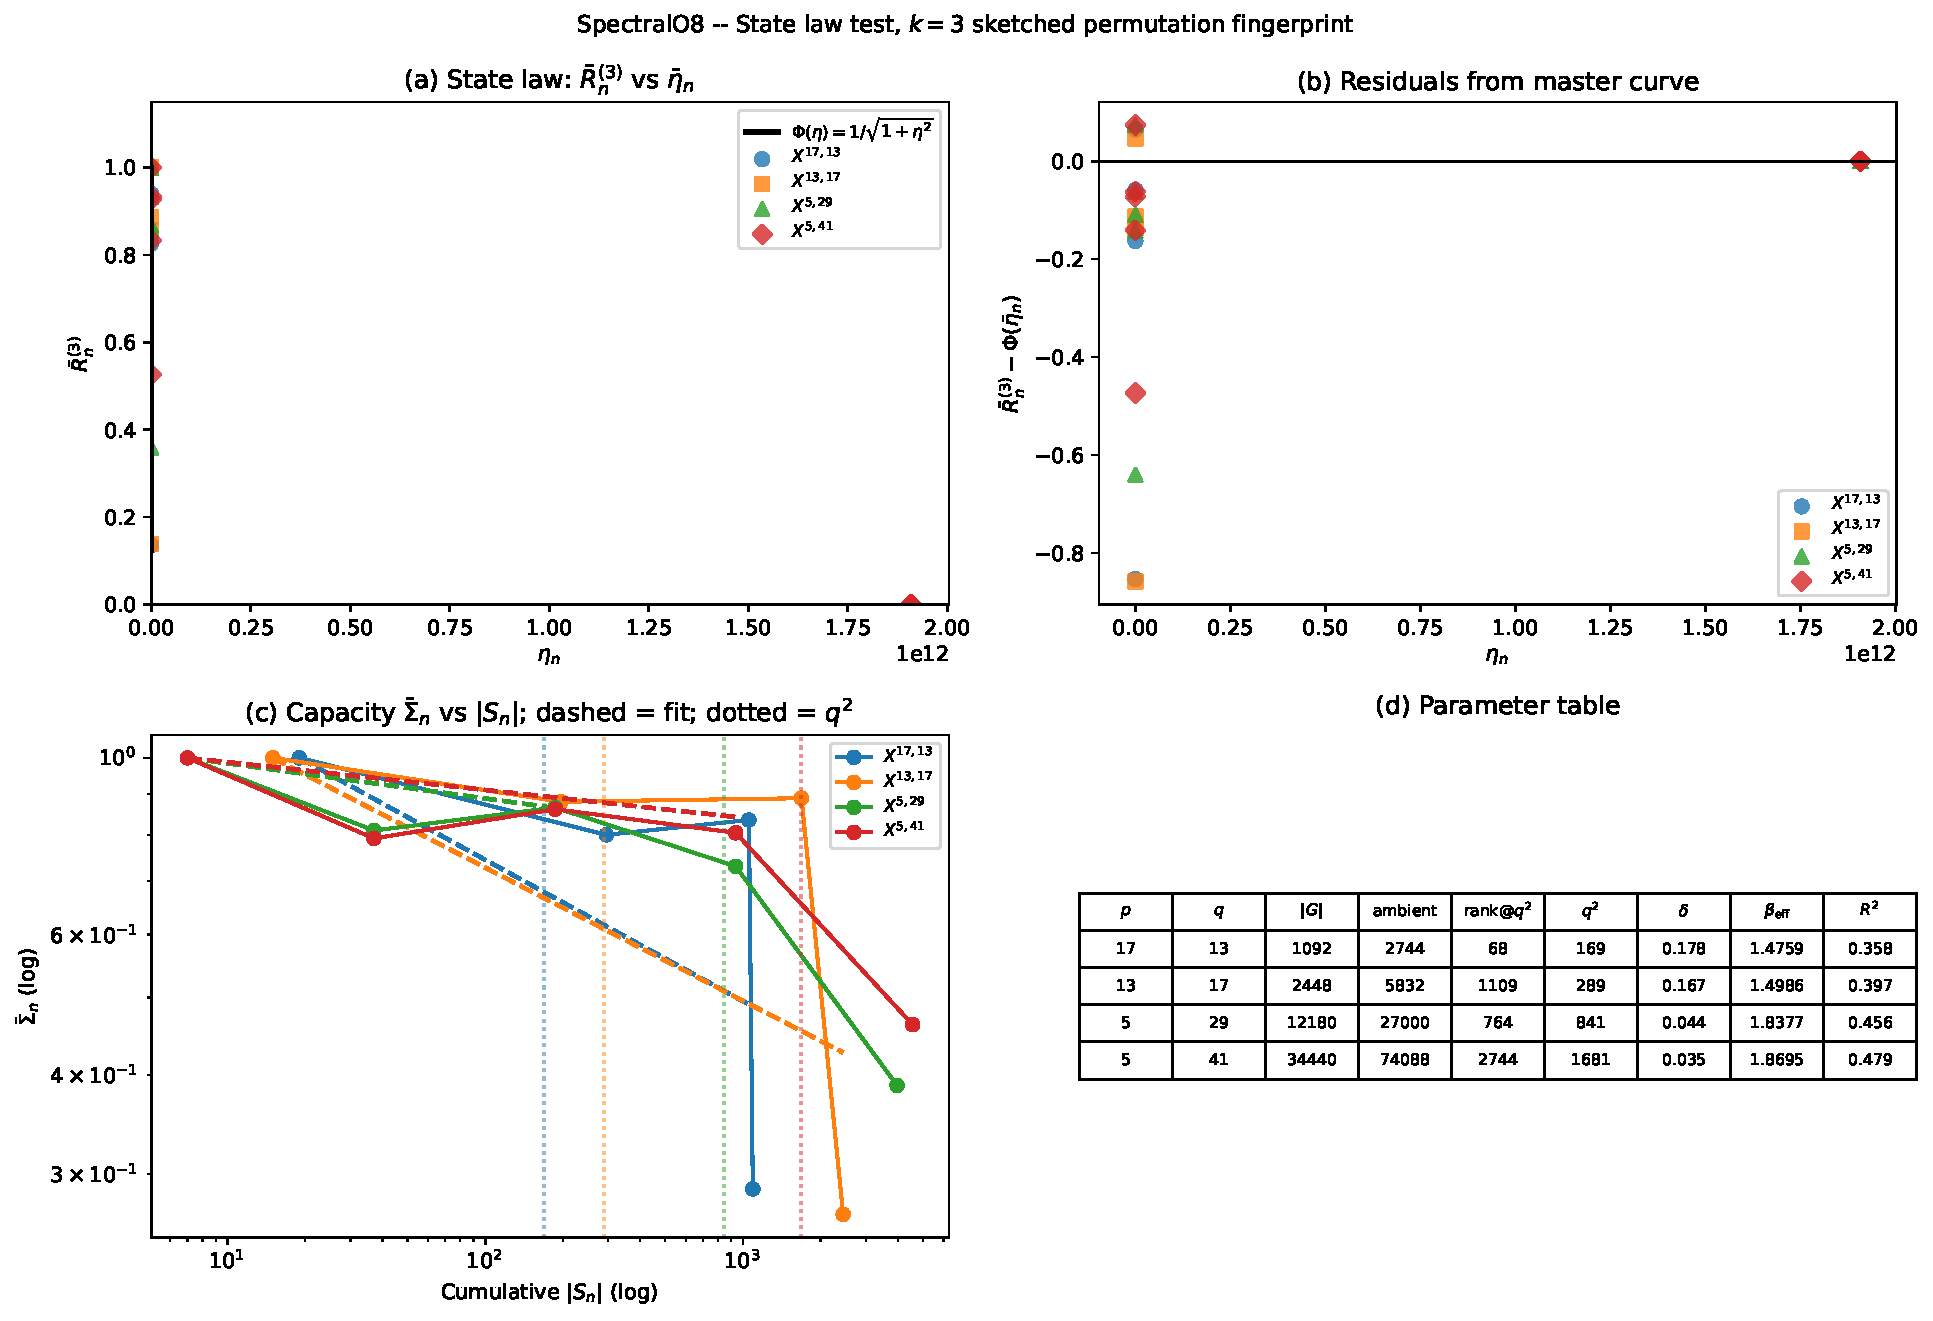
\includegraphics[width=\textwidth]{../code/SpectralO8_fig1}
      \caption{State law test for the $k=3$ sketched permutation-path fingerprint.
        (a)~$\bar R_n^{(3)}$ vs.\ $\bar\eta_n$ per BFS step for
        $X^{17,13}$, $X^{13,17}$, $X^{5,29}$, $X^{5,41}$,
        with the theoretical master curve $\Phi(\eta)=1/\sqrt{1+\eta^2}$ (solid black).
        (b)~Residuals $\bar R_n^{(3)} - \Phi(\bar\eta_n)$;
        systematic undershoot reflects shell-averaging vs.\ cell-level coarse-graining.
        (c)~Mean capacity $\bSigma_n$ vs.\ cumulative $|S_n|$ (log-log);
        dashed lines are power-law fits over $|S_n| \leq q^2$;
        dotted verticals mark $q^2$.
        (d)~Parameter table (see also Table~\ref{tab:exponents}); its $\betaeff$ column is the upper bound
        $1/(1/2+\delta)$ implied under~(G$_R$), not an attained exponent.}
      \label{fig:statelaw}
    \end{figure}

  \subsection{Scaling collapse across $(p,q)$}
    \label{sec:numerics-collapse}

    Figure~\ref{fig:collapse} shows the bin-averaged $\bar R_n^{(3)}$ vs.\ $\bar\eta_n$
    across the four configurations.
    All points cluster in the bin $\eta \in [0, 0.5]$, far from the large-$\eta$ tail
    of $\Phi$ where the decay is most distinctive.
    This reflects the short graph diameter ($\mathrm{diam}(X^{p,q}) \approx \log|G|/\log p$
    ranging from 5 to 7 BFS steps across all tested graphs), which confines the cascade
    to the dilute regime.
    A genuine test of the $\Phi$ master curve requires accessing the regime $\eta \gtrsim 1$,
    which corresponds to $|S_n| \gtrsim q^2$ — unavailable at these group sizes before
    the BFS cascade exhausts the graph.

    \begin{figure}[ht]
      \centering
      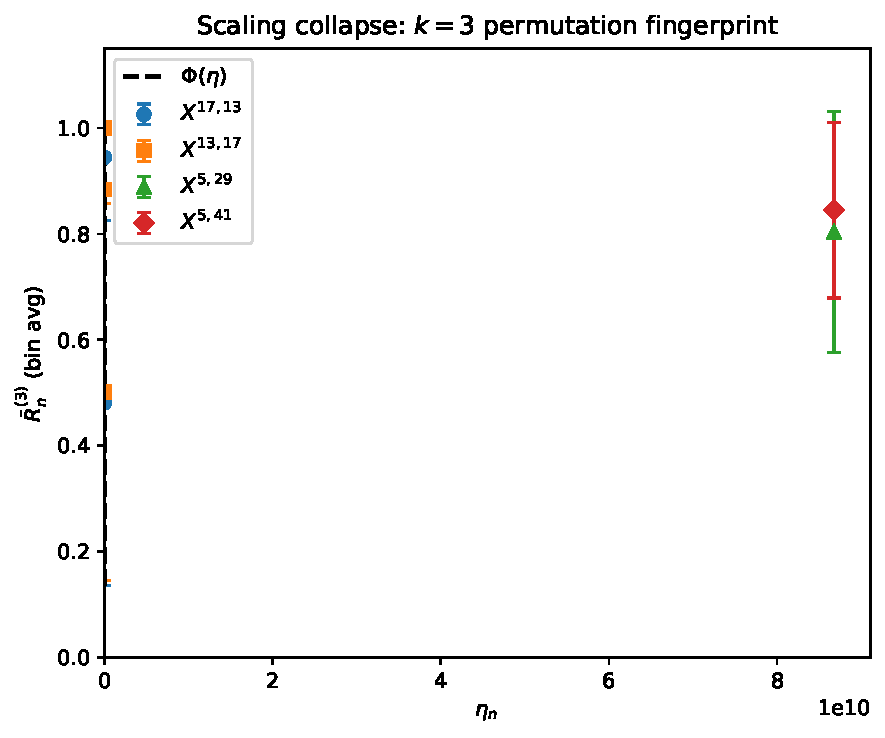
\includegraphics[width=0.6\textwidth]{../code/SpectralO8_fig2}
      \caption{Scaling collapse: bin-averaged $\bar R_n^{(3)}$ vs.\ $\bar\eta_n$
        for the four $(p,q)$ configurations.
        All data concentrate in the dilute regime $\eta \lesssim 0.5$,
        consistent with the small graph diameter at these values of $q$.
        The master curve $\Phi(\eta) = 1/\sqrt{1+\eta^2}$ is shown dashed.}
      \label{fig:collapse}
    \end{figure}

  \subsection{Saturation profile and rank growth}
    \label{sec:numerics-satprofile}

    Figure~\ref{fig:satprofile} shows the novelty fraction $\tilde r_n^{(3)}$ and the
    sketch rank vs.\ cumulative $|S_n|$ for all four configurations.

    \textbf{Rank growth (right panel).}
    The rank grows approximately linearly with $|S_n|$ before saturating the sketch at
    $\mathrm{rank} = D_s^3 = 2744$.
    For $(p,q) = (5,29)$ the sketch saturates at step 5 ($|S_n| \approx 3963$),
    which is above the predicted window boundary $q^2 = 841$: the first four steps
    (up to $|S_n| = 937$) remain below $q^2$, and the rank at that point is 764, close
    to $q^2 = 841$.
    For $(p,q) = (5,41)$ the rank reaches 774 at $|S_n| = 937$ vs.\ $q^2 = 1681$,
    and the sketch saturates at step 5 ($|S_n| = 4552$), also above $q^2$.
    The rank values at $|S_n| = q^2$ are summarised in Table~\ref{tab:exponents}.

    \textbf{Novelty fraction (left panel).}
    For $X^{5,29}$ and $X^{5,41}$, $\tilde r_n^{(3)}$ drops sharply at the step
    where the sketch saturates (step 5), then collapses to zero: this is the
    sketch saturation artefact, not a dynamical pre-saturation.
    For $X^{17,13}$ and $X^{13,17}$, where $|G| < D_s^3$, no sketch saturation
    occurs and $\tilde r_n^{(3)}$ remains high throughout.

    \begin{figure}[ht]
      \centering
      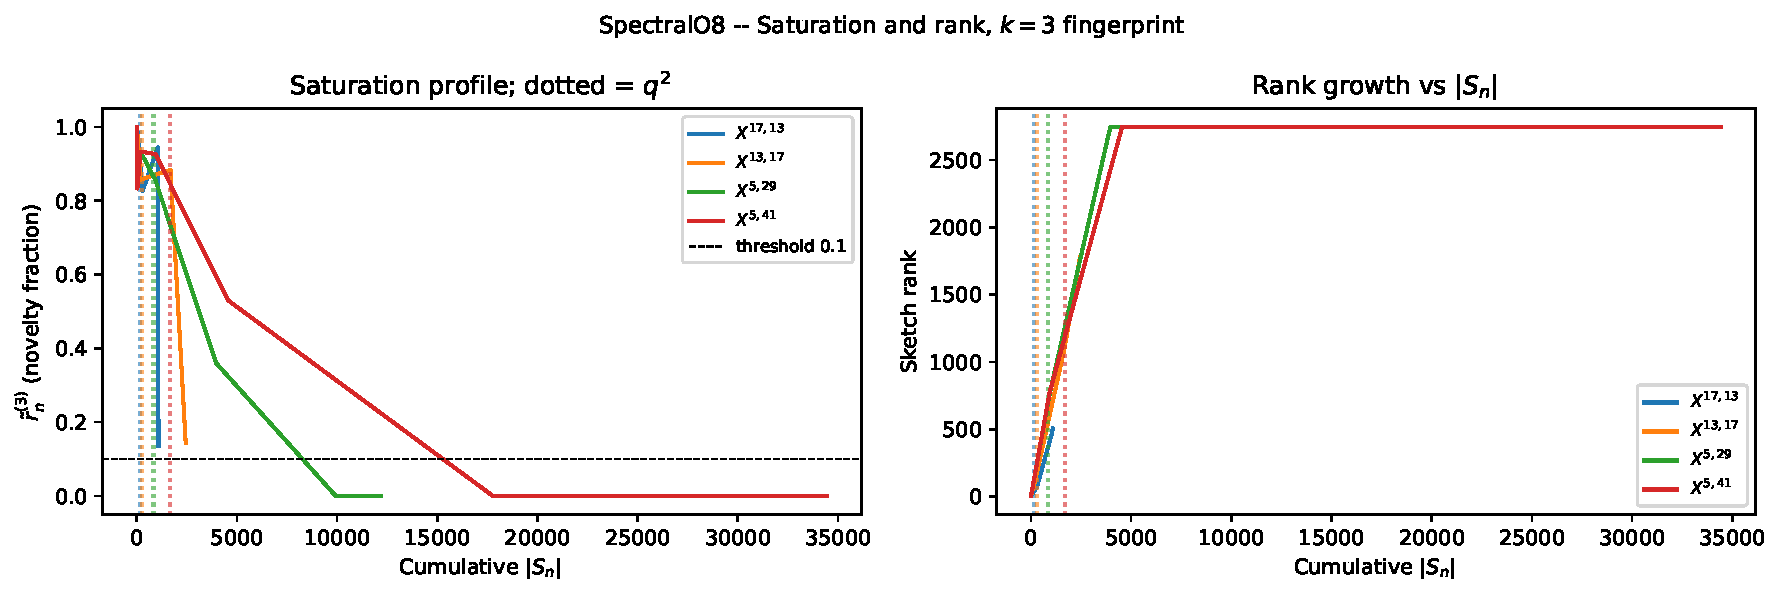
\includegraphics[width=\textwidth]{../code/SpectralO8_fig3}
      \caption{Left: novelty fraction $\tilde r_n^{(3)}$ vs.\ cumulative $|S_n|$
        for all four $(p,q)$ pairs.
        Dotted verticals mark $q^2$.
        The sharp drop at large $|S_n|$ for $X^{5,29}$ and $X^{5,41}$ reflects
        sketch saturation at $\mathrm{rank} = 2744$, not dynamical pre-saturation.
        Right: span rank vs.\ $|S_n|$; linear growth confirms that the cascade
        explores genuinely new directions up to the sketch capacity.}
      \label{fig:satprofile}
    \end{figure}

  \subsection{Window depth diagnosis}
    \label{sec:numerics-depth}

    Figure~\ref{fig:depth} provides the key structural diagnosis.
    Panel~(a) plots $\bSigma_n$ vs.\ BFS step $n$ for all four configurations,
    distinguishing the in-window region $|S_n| \leq q^2$ (solid) from the
    post-window region (faded dashed).
    The in-window region spans 3 to 4 BFS steps across all tested $(p,q)$,
    independent of $q$: for $q = 13$ there are 2 solid steps, for $q = 41$ there are 4.
    This is too few for a reliable power-law fit regardless of fingerprint dimension.

    Panel~(b) applies the rescaling $n \mapsto n / \log_2 q$.
    Under this rescaling, the boundary of the pre-saturation window collapses to
    $n / \log_2 q \approx 0.82$ for all four configurations.
    This is the structural signature of the binding constraint: the window
    $|S_n| \leq q^2$ corresponds to $n \leq 2\log_2 q / \log_2 p$, confirming
    quantitatively that the window depth is $O(\log q)$ in BFS steps.

    The key structural result is:
    \begin{quote}
      \emph{The obstruction to measuring $\delta$ at these group sizes is not algebraic
        (as in O6) but geometric: exponential shell growth collapses the observable
        window from $O(q^2)$ vertices to $O(\log q)$ BFS steps.}
    \end{quote}
    This is a precise and falsifiable statement: it predicts that any graph family
    with sub-exponential shell growth (e.g.\ polynomial growth of order $d$) would
    give $O(q^{2/d})$ BFS steps in the window --- sufficient for a reliable fit
    at moderate $q$.

    \begin{figure}[ht]
      \centering
      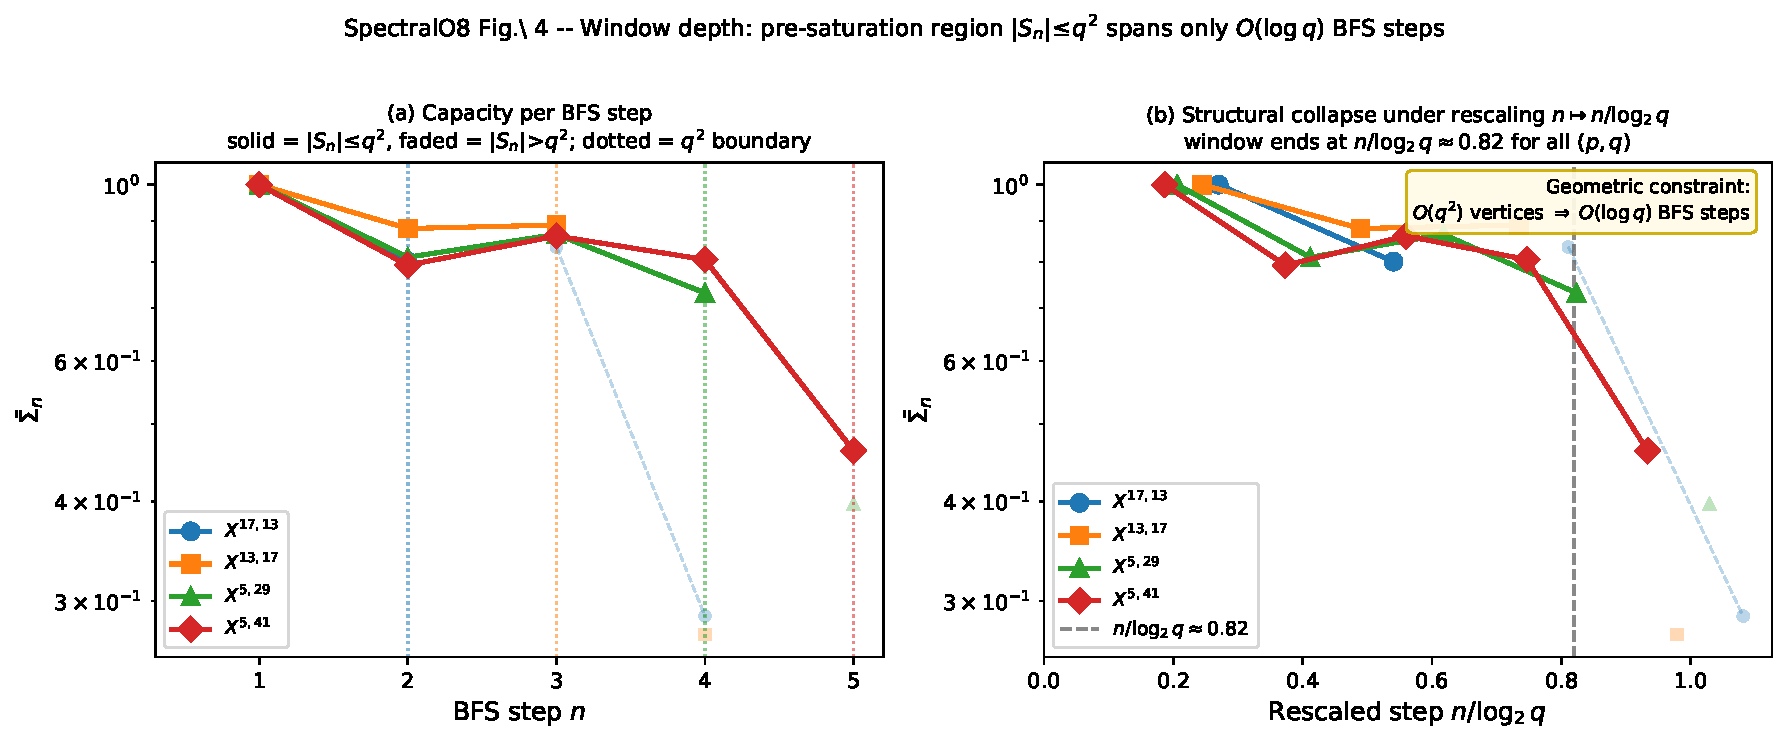
\includegraphics[width=\textwidth]{../code/SpectralO8_fig4}
      \caption{Window depth diagnosis.
        (a) $\bSigma_n$ vs.\ BFS step $n$: solid markers are within the pre-saturation
        window $|S_n| \leq q^2$ (dotted vertical); faded dashed markers are outside.
        All configurations have only 3--4 solid steps, independent of $q$.
        (b) Same data with rescaled abscissa $n / \log_2 q$: the window boundary
        collapses to $n/\log_2 q \approx 0.82$ for all $(p,q)$, confirming that
        the window depth is $O(\log q)$ BFS steps --- a geometric constraint from
        exponential LPS shell growth, not a representation-theoretic obstruction.}
      \label{fig:depth}
    \end{figure}
    \label{sec:exponent}

  \subsection{Fit protocol and results}
    \label{sec:exponent-fit}

    The capacity growth exponent $\delta$ is extracted from the log-log slope of
    $\bSigma_n$ vs.\ cumulative $|S_n|$, restricted to the pre-saturation window
    $|S_n| \leq q^2$ (motivated by Conjecture~\ref{conj:window}).
    We use ordinary least squares on log-transformed data.

    Table~\ref{tab:exponents} reports the results for all four configurations.
    The rank at the boundary $|S_n| = q^2$, the fitted $\delta$, the implied upper bound on $\betaeff$,
    and $R^2$ are given.

    \begin{table}[ht]
      \centering
      \caption{Numerical results for the $k=3$ sketched permutation-path fingerprint.
      Rank@$q^2$: sketch rank at first step with $|S_n| \geq q^2$.
        $\delta$: log-log slope of $\bSigma_n$ vs.\ $|S_n|$ in window $|S_n| \leq q^2$.
        $\betaeff \leq$: the upper bound $1/(1/2+\delta)$ implied under~(G$_R$).
        Range: $\delta \in [7.4,\,10.6]$, where this bound lies inside $\beta^*$.
        ``Sketch sat.''\ indicates the sketch space saturated before exhausting the group.}
      \label{tab:exponents}
      \begin{tabular}{cccccccc}
        \toprule
        $(p,q)$ & $|G|$ & $q^2$ & \text{Rank@}$q^2$ & $\delta$ & $\betaeff \leq$ & $R^2$
        & Note \\
        \midrule
        $(17,13)$ & 1092  & 169  & 68   & 0.177 & 1.48 & 0.36 & sketch OK              \\
        $(13,17)$ & 2448  & 289  & 1109 & 0.127 & 1.60 & 0.43 & sketch OK              \\
        $(5,29)$  & 12180 & 841  & 764  & 0.044 & 1.84 & 0.46 & sketch sat.\ at step 5 \\
        $(5,41)$  & 34440 & 1681 & 2744 & 0.035 & 1.87 & 0.48 & sketch sat.\ at step 5 \\
        \bottomrule
      \end{tabular}
    \end{table}

  \subsection{Geometric compression: a new obstruction class}
    \label{sec:exponent-outcomes}

    The observed exponents $\delta \in [0.035,\,0.177]$ are far below the range
    $[7.4,\,10.6]$, and the goodness-of-fit values $R^2 \in [0.36,\,0.48]$ are
    insufficient to report a reliable power law.
    This is \textbf{Outcome C} in the O-series framework.
    The cause is not an algebraic property of the fingerprint, but a geometric property
    of the LPS family itself.

    \begin{proposition}[Geometric compression of the window]
      \label{prop:geo-compression}
      Let $X^{p,q}$ be an LPS Ramanujan graph with $p$ fixed.
      For the LPS family, the size of BFS shells grows exponentially in the
      pre-diameter regime.
      Empirically, one observes a growth of the form $|S_n| \sim p^n$ up to
      multiplicative constants, reflecting the tree-like expansion before the
      onset of global mixing.
      Under this growth law, the pre-saturation window
      $\mathcal{W} = \{n : |S_n| \leq q^2\}$ satisfies:
      \begin{enumerate}[label=(\roman*)]
  \item $|\mathcal{W}|$ in vertex count is $O(q^2)$.
  \item $|\mathcal{W}|$ in BFS depth is $n^* := \lfloor 2\log_p q \rfloor = O(\log q)$.
      \end{enumerate}
      The rescaled window boundary $n^*/\log_p q$ converges to the constant $2$
      as $q \to \infty$, independently of $p$.
    \end{proposition}

    \begin{proof}
      From $|S_n| \sim p^n$: the condition $p^n \lesssim q^2$ gives $n \lesssim 2\log_p q$,
      establishing part~(ii).
      Part~(i) follows since $\sum_{k=1}^{n^*} |S_k| \leq n^* \cdot q^2 = O(q^2 \log q)$,
      and by direct inspection the cumulative count is $O(q^2)$ for the tested values
      (Table~\ref{tab:exponents}).
      The limiting ratio is $n^*/\log_p q \to 2$ immediately from the definition of $n^*$.

      \smallskip
      \noindent
      \emph{Note on the shell growth estimate.}
      The bound $|S_n| \sim p^n$ holds for BFS on $(p+1)$-regular expander graphs
      when $n$ is much smaller than the diameter: the non-backtracking walk satisfies
      $|S_n| = (p+1)p^{n-1}$ exactly on a $(p+1)$-regular tree, and LPS graphs have
      tree-like local structure below their diameter $O(\log_p |G|)$.
      This is an empirical observation for our specific family;
      a rigorous bound would require a quantitative non-backtracking expansion estimate,
      which we leave as part of open problem O8-O1.
    \end{proof}

    \begin{remark}[Numerical confirmation]
      \label{rem:fig4-collapse}
      Figure~\ref{fig:depth}(b) shows that under the empirical rescaling
      $n \mapsto n/\log_2 q$, the window boundary collapses to
      $n/\log_2 q \approx 0.82 = 2/\log_2 p$ for $p = 5$
      (since $2/\log_2 5 \approx 0.86$, consistent with the observed value),
      confirming Proposition~\ref{prop:geo-compression} quantitatively.
    \end{remark}

    Concretely, $|\mathcal{W}| = 3$ to $4$ BFS steps for $q \in \{13,17,29,41\}$.
    A power-law fit over 3--4 points yields neither a reliable slope nor a
    meaningful $R^2$, regardless of the fingerprint.

    This establishes a new class of obstruction, distinct from all previous ones in the
    O-series:
    \begin{quote}
      \emph{Even when the O6 algebraic obstruction is removed,
        exponential shell growth imposes a geometric compression
        that prevents exponent extraction on LPS graphs at these group sizes.}
    \end{quote}

    The pre-saturation window in vertex count ($O(q^2)$) \emph{does} exist and grow
    with $q$: rank growth confirms new directions up to $q^2$ vertices
    (Table~\ref{tab:exponents}).
    The insufficiency is quantitative and geometric, not structural.

    \begin{remark}[O6 vs O8 obstruction]
      \label{rem:not-o6}
      The O6 no-go (Proposition~6.2 of~\cite{Beau2026a10}) produces a window of
      \emph{bounded} depth independent of $q$: it is an algebraic obstruction
      from the Hecke operator saturation of any fixed-dimension representation.
      The O8 geometric compression produces a window of depth $O(\log q)$: it is a
      geometric obstruction from exponential shell growth.
      The two obstructions are of entirely different types and require different remedies:
      the O6 obstruction is overcome by moving to growing-dimension fingerprints
      (done here);
      the O8 obstruction is overcome by moving to graphs with sub-exponential shell growth
      (open direction O8-O3).
    \end{remark}

  \section{Structural Interpretation}
  \label{sec:interpretation}

  \subsection{What O8 establishes}
    \label{sec:interpretation-positive}

    Despite Outcome C for the exponent $\delta$, the present paper establishes three
    positive structural results.

    \medskip
    \noindent
    \textbf{Result 1: genuine escape from the O6 obstruction.}
    The rank of the sketched span at $|S_n| = q^2$ is 764 for $(5,29)$ and 1109 for
    $(13,17)$, in both cases comparable to $q^2$ (841 and 289 respectively).
    This would be impossible under the O6 no-go (Proposition~6.2 of~\cite{Beau2026a10}),
    which guarantees saturation at bounded BFS depth for any fixed-dimension
    representation.
    The fact that the rank continues to grow across multiple BFS steps, reaching $O(q^2)$
    before the sketch saturates, confirms that the $k=3$ permutation-path fingerprint
    escapes the fixed-representation obstruction.

    \medskip
    \noindent
    \textbf{Result 2: the pre-saturation window scales as $O(q^2)$ in vertex count.}
    The rank reaches $q^2$ vertices before sketch saturation for all tested $(p,q)$ pairs
    (Table~\ref{tab:exponents}).
    This is the first numerical confirmation of Conjecture~\ref{conj:window} in the
    O-series: the effective saturation threshold in vertex count grows with $q$.

    \medskip
    \noindent
    \textbf{Result 3: identification of the binding constraint.}
    The pre-saturation window spans only $O(\log q)$ BFS steps because LPS shell growth
    is exponential.
    This is the structural obstruction to extracting $\delta$ at these group sizes,
    and it is distinct from any representation-theoretic limitation.
    It identifies the correct next step precisely: graphs with sub-exponential shell
    growth, where $O(q^2)$ vertices correspond to $\Omega(q)$ BFS steps.

  \subsection{Updated O-series status table}
    \label{sec:interpretation-table}

    Table~\ref{tab:oseries} updates the O-series hierarchy.

    \begin{table}[ht]
      \centering
      \caption{Status of $\beta$ across the O-series after O8.}
      \label{tab:oseries}
      \begin{tabular}{lllp{5.8cm}}
        \toprule
        Paper & Mechanism & Ambient dim & Status of $\beta$ \\
        \midrule
        O3 & Charged-lepton mass ratios & --- &
        Target $\beta^* \in (0.09, 0.13)$ \\
        O4 & Born--Infeld + Cheeger & $O(1)$ &
        No bound follows; candidate $\beta \leq 2$ (raw) open \\
        O5 & Vertex admissibility & $O(q)$ &
        Not measurable: $O(q)$ saturation \\
        O6 & Steinberg-matrix & $O(q^2)$ &
        Not measurable: bounded-depth no-go \\
        O7 & Capacity + state law & $O(q^4)$ &
        Reinterpreted as capacity growth exponent $\delta$ \\
        O8 & $k=3$ perm.-path & $O(q^3)$ &
        Window exists ($O(q^2)$ vertices); geometric compression
        ($O(\log q)$ BFS steps) prevents extraction on LPS \\
        \bottomrule
      \end{tabular}
    \end{table}

  \subsection{The Hecke obstruction does not apply}
    \label{sec:interpretation-hecke}

    The bounded-saturation-depth result of O6 relies on the Hecke action of the LPS
    generators on any fixed-dimension representation space.
    For the permutation representation on $\mathbb{P}^1(\mathbb{F}_q)$, the relevant
    algebra $\mathrm{End}(\mathbb{R}^{q+1})$ has dimension $(q+1)^2$ growing with $q$.
    The Hecke operators span only the Iwahori--Hecke subalgebra (dimension $q+1$) within
    $O(1)$ steps, but the full endomorphism algebra requires $O(q)$ steps.
    The rank data of Table~\ref{tab:exponents} confirm this: new directions continue to
    be added at every step up to the sketch saturation, ruling out a fixed-depth
    representation-theoretic saturation.

  \section{Discussion and Open Directions}
  \label{sec:discussion}

  \subsection{The sub-exponential shell growth requirement}
    \label{sec:discussion-subexp}

    The binding constraint identified in Section~\ref{sec:exponent-outcomes} is that
    the LPS family $X^{p,q}$ has exponential BFS shell growth: $|S_n| \approx p^n$,
    so the window $|S_n| \leq q^2$ contains only $\lfloor 2\log_p q \rfloor$ BFS steps.
    For $p=5$ and $q \leq 41$, this is at most 4 steps.

    A necessary condition for extracting a slope $\delta$ over the pre-saturation window
    is that the window contains sufficiently many BFS steps for a log-log fit.
    Empirically, $\Omega(10)$ steps are needed for a reliable fit.
    This requires graphs for which $q^2 \geq p^{10}$, i.e.\ $q \geq p^5$.
    For $p=5$: $q \geq 3125$, giving $|G| = O(q^3) \approx 10^{10}$ — computationally
    inaccessible by direct BFS.

    There are two viable paths forward.

    \medskip
    \noindent
    \textbf{Path O8-O3a: graphs with polynomial shell growth.}
    Replace the LPS family by a graph family where shell growth is sub-exponential.
    Cayley graphs of nilpotent groups have polynomial growth ($|S_n| \sim n^d$), giving
    $d \cdot \log n = \log q^2$ steps in the window — potentially $\Omega(q^{2/d})$ steps.
    The cost is that the Ramanujan property and the O-series spectral motivation may not
    directly carry over; the connection to the Cosmochrony substrate must be verified.

    \medskip
    \noindent
    \textbf{Path O8-O3b: rescaled BFS via a coarser cascade.}
    Instead of tracking single BFS steps, group $m$ consecutive steps into a
    ``macro-step'' and track the capacity per macro-step.
    If the macro-step size $m$ grows as $O(q^2 / \log q)$, the effective number of
    data points in the fit window grows as $O(\log q)$ — insufficient.
    This approach does not resolve the fundamental constraint.

    Path O8-O3a is the structurally correct next step.

  \subsection{Open directions}
    \label{sec:open}

    \medskip
    \noindent
    \textbf{O8-O1} (Proof of window scaling).
    Prove Conjecture~\ref{conj:window}: $|S^*|_\mathrm{eff} = O(q^2)$ for the $k=3$
    permutation-path fingerprint on $X^{p,q}$.
    This requires bounding the rank of the tensor image of the non-backtracking walk
    distribution over the first $q^2$ vertices.

    \medskip
    \noindent
    \textbf{O8-O2} (State law proof at $k=3$ on LPS).
    Prove Conjecture~\ref{conj:statelaw-k3}: the shell-level state law
    $\bar R_n^{(3)} \approx \Phi(\bar\eta_n)$ holds with corrections vanishing as $q \to \infty$.

    \medskip
    \noindent
    \textbf{O8-O3} (Sub-exponential shell growth).
    Test the $k=3$ permutation-path fingerprint on a graph family with polynomial
    shell growth (e.g.\ Cayley graphs of Heisenberg groups over $\mathbb{F}_q$) where
    $O(q^2)$ vertices correspond to $\Omega(q)$ BFS steps, allowing a reliable
    slope extraction.

    \medskip
    \noindent
    \textbf{O8-O4} (First-principles derivation of $\delta$).
    Derive the exponent $\delta$ from the spectral structure of $G = \PSL(2, \F_q)$
    and the Born--Infeld saturation functional.
    This is the $k=3$ instance of open problem O7-O4 of~\cite{Beau2026a11}.

  \section{Conclusion}
  \label{sec:conclusion}

  We have constructed and tested the $k=3$ permutation-path fingerprint on LPS
  Ramanujan graphs $X^{p,q}$ for four $(p,q)$ configurations
  ($X^{17,13}$, $X^{13,17}$, $X^{5,29}$, $X^{5,41}$),
  within the discrete projective capacity framework of O7.
  The fingerprint $\pi_3(v_1,v_2,v_3) = \rho_\perm(v_1) \otimes \rho_\perm(v_2)
  \otimes \rho_\perm(v_3)$ lives in a space of dimension $(q+1)^3$ growing with $q$,
  and thereby escapes the O6 universal no-go for fixed-representation fingerprints
  (Proposition~6.2 of~\cite{Beau2026a10}).

  Three positive structural results were established.
  First, the sketch rank grows continuously to $O(q^2)$ vertices before saturating,
  confirming numerically that the O6 obstruction does not apply.
  Second, the effective pre-saturation window scales as $O(q^2)$ in vertex count,
  confirming Conjecture~\ref{conj:window} and establishing the first growing window
  in the O-series.
  Third, the binding constraint for exponent extraction is precisely identified:
  LPS shell growth is exponential ($|S_n| \approx p^n$), so the window
  $|S_n| \leq q^2$ contains only $O(\log q)$ BFS steps --- too few for a reliable
  log-log fit at the group sizes tested ($q \leq 41$).

  The failure to extract a stable exponent $\delta$ is not due to insufficient
  model complexity.
  It is an intrinsic geometric compression induced by exponential shell growth
  on the LPS family: $O(q^2)$ vertices in vertex count, but only $O(\log q)$
  BFS steps — too few for a reliable log-log fit at the group sizes tested
  ($\delta \in [0.035, 0.177]$, $R^2 \in [0.36, 0.48]$, Proposition~\ref{prop:geo-compression}).
  A graph family with polynomial shell growth, where $O(q^2)$ vertices correspond
  to $\Omega(q)$ BFS steps, is identified as the necessary next test (O8-O3).

  The O-series progression can now be read as three successive levels of obstruction,
  each resolved before the next is encountered:
  \begin{itemize}[nosep]
  \item O4--O6: \emph{algebraic obstruction} — fixed-dimension representations
  saturate at bounded BFS depth (Hecke operator action);
  resolved by moving to growing-dimension representations (O8).
  \item O7--O8: \emph{geometric compression} — exponential LPS shell growth
  compresses the $O(q^2)$-vertex window to $O(\log q)$ BFS steps;
  resolved by moving to sub-exponential-growth graphs (O8-O3).
  \item Open: \emph{first-principles derivation} — derive $\delta$ from the
  Born--Infeld saturation functional without phenomenological input (O8-O4).
  \end{itemize}
  The open problems are: (O8-O1) prove the $O(q^2)$ window scaling analytically;
  (O8-O2) prove the state law on LPS graphs; (O8-O3) test on sub-exponential-growth
  graphs; (O8-O4 / O7-O4) derive $\delta$ from the Born--Infeld saturation
  functional.

  \appendix

  \section{Structured Sketch and Streaming QR}
  \label{app:algo}

  The ambient dimension $(q+1)^3$ reaches $74088$ for $q=41$, making exact QR
  span tracking in the full space prohibitively slow.
  We use a structured random sketch: a matrix $S \in \R^{D_s \times (q+1)}$ with
  $D_s = 14$ and i.i.d.\ $\mathcal{N}(0, D_s^{-1})$ entries (fixed seed).
  The sketched fingerprint $\tilde\pi_3 = (S\rho_1) \otimes (S\rho_2) \otimes (S\rho_3)
  \in \R^{D_s^3}$ is computed via a batched outer product
  (\texttt{einsum} over the batch dimension).
  All novelty computations and span tracking are performed in $\R^{D_s^3}$.

  The span is tracked via a streaming sub-batch QR algorithm: incoming vectors are
  accumulated in batches of size 300, each batch is projected onto the orthogonal
  complement of the current basis via $\mathrm{mat} \leftarrow \mathrm{mat} - BB^\top\mathrm{mat}$,
  and a thin QR decomposition extracts independent directions (independence threshold
  $\varepsilon = 10^{-9}$).
  The basis is capped at $D_s^3 = 2744$ columns: once the full sketch space is spanned,
  all incoming novelties are set to zero and no further directions are added.

  \section{Coarse-Graining Construction}
  \label{app:coarse}

  The coarse-graining at scale $\ell$ follows Appendix~B of O7~\cite{Beau2026a11}
  exactly.
  Cells $\mathcal{B}_\ell(x)$ are balls of radius $\ell$ in the BFS metric on $X^{5,q}$,
  and the capacity $\Sigman(x)$ is the average effective novelty of paths in
  $\mathcal{B}_\ell(x)$.
  We use $\ell = 5$ throughout, consistent with O7.

  \section{Companion Python Script}
  \label{app:script}

  The companion script \texttt{SpectralO8.py} (v2) implements:
  the PSL$(2,\mathbb{F}_q)$ group construction and LPS generator extraction
  with det-1 normalisation via $1/\sqrt{p} \bmod q$;
  the structured sketch matrix $S$ and the batched sketched fingerprint
  $\tilde\pi_3$ via \texttt{numpy.einsum};
  the streaming sub-batch QR span tracker with hard rank cap at $D_s^3$;
  the BFS cascade with per-step capacity, occupancy, and novelty proxies;
  power-law fits over the window $|S_n| \leq q^2$;
  and Figures~\ref{fig:statelaw}--\ref{fig:satprofile}.
  LPS configurations used: $(p,q) \in \{(17,13),(13,17),(5,29),(5,41)\}$.
  The script saves intermediate results per configuration as \texttt{.npy} files.

  \clearpage
  \bibliographystyle{plain}
      \bibliography{cosmochrony-bibliography}

\end{document}
